\documentclass[tikz,border=4pt]{standalone}
\usepackage{mathptmx}\usepackage{amssymb,amsmath}
\usetikzlibrary{positioning,arrows.meta,fit,backgrounds,calc}
\definecolor{ink}{HTML}{1F2A36}
\definecolor{rblue}{HTML}{2B6CB0}
\definecolor{rfill}{HTML}{EAF2FB}
\definecolor{gfill}{HTML}{F4F5F7}
\definecolor{vfill}{HTML}{FFF4E5}
\definecolor{vedge}{HTML}{C76E00}
\begin{document}\hyphenpenalty=10000\exhyphenpenalty=10000
\begin{tikzpicture}[
  font=\small, >={Stealth[length=2.6mm,width=2mm]},
  box/.style={draw=ink, line width=0.6pt, rounded corners=2pt, fill=gfill, align=center,
              minimum height=21mm, text width=26mm, inner sep=2pt},
  rbox/.style={box, draw=rblue, fill=rfill},
  vbox/.style={box, draw=vedge, fill=vfill},
  arr/.style={->, line width=0.8pt, draw=ink},
  lbl/.style={font=\scriptsize\itshape, text=ink!75},
  node distance=7mm]

\node[box, text width=21mm] (in) {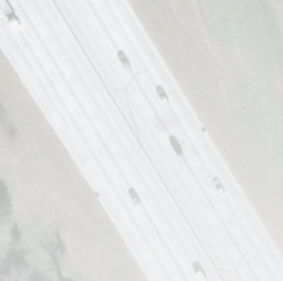
\includegraphics[width=15mm]{t_haze.png}\\[1pt]\textbf{Input image} (hazy)};
\node[rbox, right=of in] (feat) {\textbf{Image statistics}\\[2pt]$\mathbf{f}(x)\in\mathbb{R}^{11}$\\[1pt]{\scriptsize luminance, dark channel,\\ contrast, entropy, noise}};
\node[rbox, right=of feat] (det) {\textbf{Degradation\\detector}\\[2pt]{\scriptsize GBDT or two thresholds}\\[1pt]$\hat c\in\{\text{clean},\text{haze},\text{low}\}$};
\node[rbox, right=of det] (lut) {\textbf{Lookup table}\\[2pt]$a^{*}(\hat c)$\\[2pt]{\scriptsize clean$\to$none/$\gamma$\\ haze$\to$DCP\quad low$\to\gamma$}};
\node[box, right=of lut, text width=21mm] (enh) {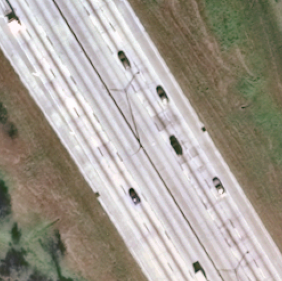
\includegraphics[width=15mm]{t_dehaze.png}\\[1pt]\textbf{Enhanced image}};
\node[vbox, right=of enh, text width=22mm] (vlm) {\textbf{Frozen VLM}\\[2pt]{\scriptsize Qwen2.5-VL-3B /\\ Qwen2-VL-2B}\\[2pt]{\scriptsize one forward pass}};
\node[box, right=7mm of vlm, text width=15mm, minimum height=12mm] (ans) {\textbf{Answer}\\{\scriptsize $P(\text{yes})$ or A--D}};

\foreach \a/\b in {in/feat, feat/det, det/lut, lut/enh, enh/vlm, vlm/ans} \draw[arr] (\a) -- (\b);

\node[box, below=11mm of vlm, minimum height=10mm, text width=22mm] (q) {\textbf{Question} $q$\\{\scriptsize scene, surface, object}};
\draw[arr] (q) -- (vlm);

\node[box, draw=ink!60, dashed, fill=white, below=11mm of det, xshift=17mm, text width=78mm, minimum height=10mm] (off)
  {\textbf{Offline, once per VLM:} accuracy of each operator per condition on training questions $\Rightarrow a^{*}(c)$};
\draw[arr, dashed, draw=ink!70] (off.north -| lut) -- (lut.south);

\begin{scope}[on background layer]
\node[draw=rblue, dashed, line width=0.7pt, rounded corners=4pt, fill=rblue!3, inner xsep=3mm, inner ysep=3mm,
      fit=(feat)(det)(lut), label={[text=rblue, font=\small\bfseries]above:Router (CPU only, 15--28\,ms per image, no VLM call)}] (grp) {};
\end{scope}

\end{tikzpicture}
\end{document}
